\documentclass[a4paper,10pt]{report}
\usepackage[utf8x]{inputenc}
\usepackage[francais]{babel}
\usepackage[T1]{fontenc}
\usepackage{graphicx}
\usepackage[colorlinks=true, urlcolor=blue, linkcolor=black]{hyperref}

% Title Page
\title{Web Game Engine - Cahier des charges}
\author{Ilyas Boutebal \and Maxime Colin \and Adrian Gaudebert \and Youness Hamri \and Van-Duc Nguyen}

\begin{document}
\maketitle

\tableofcontents

\chapter{Contexte}

\subsection{Fightly}

Le projet dans sa version initiale consistait à développer un jeu au tour par tour, par navigateur sur internet appelé Fightly, mais plusieurs raisons nous ont amener à ne pas prendre en compte des parties du jeu que nous avons estimé sortant du cadre du Master, notamment les aspects graphiques, vidéo, audio, forum de discutions et l'initialisation des parties. Le projet est donc réduit à l'essentiel, c'est à dire fournir un moteur de jeu qui permet d'implémenter les fonctionnalités de tout ce qui est en lien avec le déroulement du jeu. Autrement dit, on se limitera à la mécanique du jeu.

Fightly est un projet de jeu qui se déroule sur une carte choisie au hasard parmi un ensemble de cartes précrées. Les cartes sont composées de cases hexagonales contigues où chacune possède un type de terrain particulier ralentissant ainsi ou intérdisant les déplacement sur certains types de terrains. Les joueurs choisisent leurs unités de combats composées de fantassins, archers et chevaliers ayant chacuns des caractéristiques et des capacités différentes. Ils les placent sur la carte, et s'affrontent chacun son tour en les faisant déplacer et attaquer suivant des règles de portée bien précises.

\section{Le Jeu vidéo}
Le marché du jeu vidéo s’est beaucoup développé depuis l’arrivée de l’ancêtre Pong ou du célèbre Tetris. On joue aujourd’hui à des jeux de plus en plus beaux, demandant de plus en plus de ressources à nos machines. Mais on voit aussi d’autres utilisations du jeu vidéo arriver : le Serious Gaming, par exemple, est une branche en pleine expansion en ce moment. Le Social Gaming également, représenté activement par les nombreux jeux basés sur Facebook et ses possibilités en terme de diffusion.

Si on s’essayait à une catégorisation rapide des jeux vidéo, voici ce qui pourrait ressortir : les jeux consoles, les jeux PC “classiques”, les jeux en ligne (MMO en tous genres compris). Dans cette dernière catégorie, on trouve beaucoup de types de jeux différents : les MMO dans le genre de World of Warcraft, les jeux multijoueur comme Counter Strike ou Team Fortress, les modes multi des jeux principalement solo, et les jeux par navigateur.

\section{Les jeux par navigateur}
Le jeu par navigateur, ou Browser Game en anglais, se joue par définition dans un navigateur Internet. On retrouve donc dans cette catégorie les jeux “Facebook” cités plus haut, la majorité des jeux en Flash, mais également un très grand nombre de jeux que nous appellerons les Jeux Web, puisqu’ils se basent sur les technologies du Web ouvert. Quelques exemples de jeux web relativement connus : Ogame, Travian, ou le français Hordes.

Ces trois exemples ne sont cependant pas représentatifs de la diversité que l’on trouve dans les jeux web. Les jeux d’élevage virtuel, par exemple, sont extrêmement nombreux sur le Web. À quoi est due cette profusion de jeux web ? Majoritairement à la simplicité d’accès du développement web. Faire un jeu web, en soit, c’est développer un site web. Or, avec des technologies très répandues comme PHP, HTML et CSS, avec toutes les ressources que l’on trouve autour de ces dernières (il suffit de regarder les tutoriels du Site du Zéro pour s’en rendre compte), il est très simple pour une personne un peu motivée de créer son propre jeu web.

Malheureusement, s’il est simple de créer un jeu web “basique”, les développeurs sont rapidement limités par les technologies qu’ils utilisent. Il est quasiment impossible de faire du temps réel avec PHP, le couple HTML / CSS n’est pas adapté à l’affichage d’effets spéciaux ou d’animations complexes, et si l’arrivée récente de frameworks JavaScript comme jQuery a permis de repousser un peu ces limites techniques, cela ne résout pas le problème.

\section{Les technologies du web}
Il existe une solution simple aux limitations techniques actuelles des technologies web : se tourner vers le futur et utiliser de nouvelles technologies, pas encore éprouvées, mais qui permettent d’aller beaucoup plus loin dans la création de nos jeux web.

HTML 5, la nouvelle mouture du langage de description des pages web, apporte au développeur un très grand nombre de fonctionnalités clés : le temps réel dans le navigateur avec les WebSockets, les manipulations graphiques avancées avec le SVG et les Canvas, la vidéo et le son avec Video et Audio, et bien d’autres.

La version 3 du langage CSS offre elle aussi d’alléchantes nouveautés : les animations, les transitions, les polices particulières, ainsi que tous les effets graphiques amplement simplifiés.

\chapter{Le projet}

\section{Objectifs}

Toutes les avancées actuelles du web ouvrent indéniablement les portes à des jeux de plus en plus impressionnants, de plus en plus profonds, le tout se passant dans un navigateur ! Il faudra cependant du temps pour que les développeurs maîtrisent tout ceci, pour que des outils facilitant l’utilisation de ces technologies apparaissent, et donc pour que l’accès à toutes ces possibilités pour nos jeux devienne simple.

Voici donc où se place ce projet : notre objectif est de fournir un outil complet, permettant de créer de façon simple et rapide un jeu profitant des dernières avancées en matière de technologie web. Il constitura un ensemble d'outils qui fournissent un cadre de développement et des fonctionnalités permettant d'implémenter tout ou partie d'un jeu.

Le moteur sera prioritairement conçu pour des jeux de stratégie au tour par tour. On cherchera à le rendre aussi générique que possible, afin de permettre une grande diversité dans les types de jeux développables avec notre outil. On veillera aussi à faciliter l'extensibilité du projet, toujours dans le but d'offrir la possibilité d'en étendre facilement les fonctionnalités.

Un des objectifs secondaires du projet est d'utiliser des technologies récentes et innovantes. Si la compatibilité avec les différents navigateurs du marché doit être un facteur important, elle ne doit pas être une limitation dans le choix des outils à utiliser. 

Pour finir, ce projet sera libre, c'est-à-dire qu'il sera distribué sous licence libre, et qu'à terme on voudra mettre en place une communauté autour du développement de ce produit. 

\section{Les jeux de stratégie au tour par tour}

Présentation de plusieurs jeux STpT. Diagrammes de classes. 

On en sort les grands concepts suivants... 

Modélisation du gameplay

\section{Spécifications}

\subsection{Moteur de jeu}

Le moteur de jeu se découpe en deux parties : côté serveur, on gère les règles du jeu, le gameplay, et les joueurs. 

Côté client, on gère l'affichage et les actions utilisateur. 

\subsection{Serveur}

Le serveur sera la partie du moteur qui fera tourner les parties et permettra la communication et les interraction entre les joueurs. Il aura pour rôle de contrôler les parties, lier les clients et gérer leur actions. Il aura également le rôle d'arbitre dans une partie. 

Le serveur sera séparer en deux grandes parties : Une partie Noyau et une partie Monde.

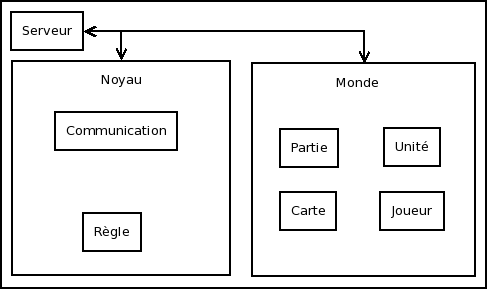
\includegraphics{img/server-organisation.png}

\subsubsection{Package Noyau}

La partie Noyau du serveur gère les fonctionnalités de base du moteur. Elle contient un ensemble de modules qui sont a priori indépendant du type de jeu implémenté. De plus, ce noyau doit permettre les interactions entre les règles et les modules de la partie Monde, quels que soient ces derniers. 

La sous-partie communication du serveur doit permettre d'envoyer et de recevoir des messages. Cette partie devra également accepter et gérer les connexions clients.

La sous-partie protocole sera charger d'adapter les messages. C'est à dire encapsuler nos message dans le protocole choisi pour l'envoie de message et extraire le contenu d'un message reçu. Il fera le lien entre les messages sur le réseaux et les messages comprehensibles par le client et le serveur.

La sous-partie règles sera charger de stocker et traiter les règles du jeu. Elle contiendra des fonctionnalités permetant de créer une base de règles. Ces règle pourront être ajouté et supprimé individuellement ou charger à partir d'un fichier de règle. La partie règle devra également valider (ou invalider) les requêtes du client.

\subsubsection{Package Monde}

La partie Monde est totalement dynamique : les modules qu'elle contient sont fonction du jeu à développer, et peuvent donc changer du tout au tout. Les modules de cette partie doivent donc pouvoir être appelés depuis le noyau sans avoir à faire autre chose que de la configuration. 

Les modules présents dans cette partie implémentent des fonctionnalités du jeu. Ceux choisis ici sont donc ceux qui serviront, a priori, au jeu Fightly.

Cette partie aura des fonctionnalités permettant de gérer une partie. Ces fonctionnalité concerneront le chargement et la sauvegarde d'une partie. Elle gera également la connexion et la déconnexion à une partie.

Une sous-partie sera dédié à la gestion de la carte. Elle ne disposera que d'une seule fonctionnalité permettant de charger la carte à partir d'un fichier.

Le serveur disposera de fonctionnalités pour gérer les unités des joueurs. Cette sous-partie permettra de créer, supprimer ou déplacer les unités.

Le serveur devra également gérer les joueurs. Une sous-partie permmettra de créer et supprimer des joueurs dans une partie. Elle devra également gerer l'abandon d'un joueur durant une partie. C'est à dire retirer le joueur et ses unités de la partie.

\subsection{Client}

Le client doit gérer l'affichage (et éventuellement la gestion du son), la réception de données envoyées par le serveur, et les données entrées par le joueur (inputs) et l'envoi des demandes de modification des données (modification du monde).

\subsubsection{Affichage}

Pour l’affichage, La partie client de notre moteur de jeux ne dispose que les données d’une partie de la carte, c’est la zone ou le périmètre des unités du joueur. A chaque déplacement d’unité, le client doit demander au serveur de charger la partie  correspondante de la carte.

La carte est représentée sous forme de cellules (rectangulaire ou hexagonale) de plusieurs types (montagne, foret, chemin, mer …), chaque cellule a des propriétés (accessibilité : oui ou non par une unité par exemple).

Deuxième grand élément du jeu c’est les unités, le client dispose d’un ensemble de fonctionnalités capable de : Créer, déplacer et mettre a jour les propriétés de ces unité ainsi que la suppression d’une unité (après une éventuelle déconnexion).

\subsubsection{Input}

Cette partie s'occupe de la lecture des périphériques externes comme :

- La Souris (lecture de l'état des boutons (clics) et de la position).

- Le Clavier (de l'état des boutons).

Ces Inputs seront utilisés directement par les fonctionnalités de

\subsubsection{Communication}

Le client doit être capable d’établir une connexion avec le serveur après l’identification du joueur, il peut également établir des connexions avec les autres clients pour échanger des messages (le Chat par exemple).

\subsubsection{Protocole}

Pour la communication des données, la partie « client » du moteur de jeux doit transformer les messages ou les requêtes dans un format donné (XML ou JSON par exemple) pour les envoyer au serveur, elle doit être capable aussi d’interpréter les messages qui viennent de ce dernier.

Un protocole de communication bidirectionnel sera utilisé par le client et le serveur (Websocket par exemple), ce protocole permet la notification au client d’un changement d’état du serveur ainsi que l’envoie de données en mode poussé au serveur.

\subsubsection{Règles}

Le client dispose d’une base de règles et une fonction, qui lui permettent de valider ou interdire des actions ou des requêtes demandées par le joueur. (par exemple le déplacement d’une unité vers une cellule inaccessible).

\subsubsection{Monde}

Dans cette partie du moteur, on trouve toutes les fonctions qui correspondent aux différentes actions. C'est elle qui se chargera de la modification du monde. On prend comme exemple le déplacement d’une unité ; quand on clique sur une unité, cela nous permet de voir tous les endroits (cellules) où on peut faire déplacer cette unité. Au deuxième clique l’unité est déplacé vers la cellule sélectionné, ensuite le client doit envoyer une demande de modification de position (x,y) de cette unité au serveur.

\end{document}
